\documentclass[12pt, a4paper]{article}
\usepackage[utf8]{inputenc}
\usepackage[english,russian]{babel}
\usepackage{graphicx}
\usepackage{wrapfig}
\usepackage[left=2cm,right=1.5cm,top=1.5cm,bottom=1.5cm]{geometry}

\begin{document}
\thispagestyle{empty}

\includegraphics[scale=0.75]{itmo.png}

\begin{tabular}{l l}
	Группа P3110 & \hspace{1.5cm}Дата и время измерений 11.01.2020 19:00\\
	Студент Бавыкин Роман & \hspace{1.5cm}Работа выполнена\\
	Преподаватель Коробков М.П. & \hspace{1.5cm}Отчет принят
\end{tabular}

\begin{center}
	\large
	\textbf{Рабочий протокол и отчет по\\
		лабораторной работе №1.24V}\\
	Оборотный маятник Катера\\
\end{center}
\begin{enumerate}
	\item Цель работы.
	\begin{itemize}
		\item Изучить колебательное движение тела на примере оборотного маятника.
		\item Определить ускорение свободного падения тел.
	\end{itemize}	
	\item Задачи, решаемые при выполнении работы.
	\begin{itemize}
		\item Измерить периоды $T_1$ и $T_2$ для каждого положения груза $M_1$ не менее 5 раз
		\item Построить графики зависимостей $<T_1(x_2)>$ и $<T_1(x_2)>$, определить положения $x_2$ и $x'_2$, где $\left\langle T_1\right\rangle=\left\langle T_2\right\rangle$.
		\item Вычислить ускорение свободного падения и определить его погрешность.
	\end{itemize}
	\item Объект исследования.
	
	Оборотный маятник Катера.
	\item Метод экспериментального исследования.
	
	Прямые многократные измерения, построение графиков зависимости, интерполяция значений, вычисление значений и нахождение абсолютной и относительной погрешностей.
	\item Рабочие формулы и исходные данные.
	$$\left\langle T\right\rangle=\frac1N\sum_{i=1}^{N}t_i;$$
	$$l_{\mbox{пр}}=x_2+x`_2;$$
	$$g=\frac{4\pi^2l_{\mbox{пр}}}{T^2};$$
	$$\epsilon_g=\frac{\Delta_g}g=\sqrt{{\left(\frac{2\Delta T}T\right)}^2+{\left(\frac{\Delta l_{\mbox{пр}}}{l_{\mbox{пр}}}\right)}^2}.$$
	$$\Delta T=0,1\mbox{мс};\ \Delta l_{\mbox{пр}}=1\mbox{мм}$$
	\item Измерительные приборы.
	
	\begin{tabular}{|c|c|c|c|c|}
		\hline
		№ &  &  & Используемый & Погрешность \\
		п/п & Наименование & Тип прибора & диапазон & прибора \\
		\hline
		1 & Секундомер & Электронный & 0--10000мс & 0,1мс\\
		\hline
	\end{tabular}
	\newpage
	\item Схема установки.
	
	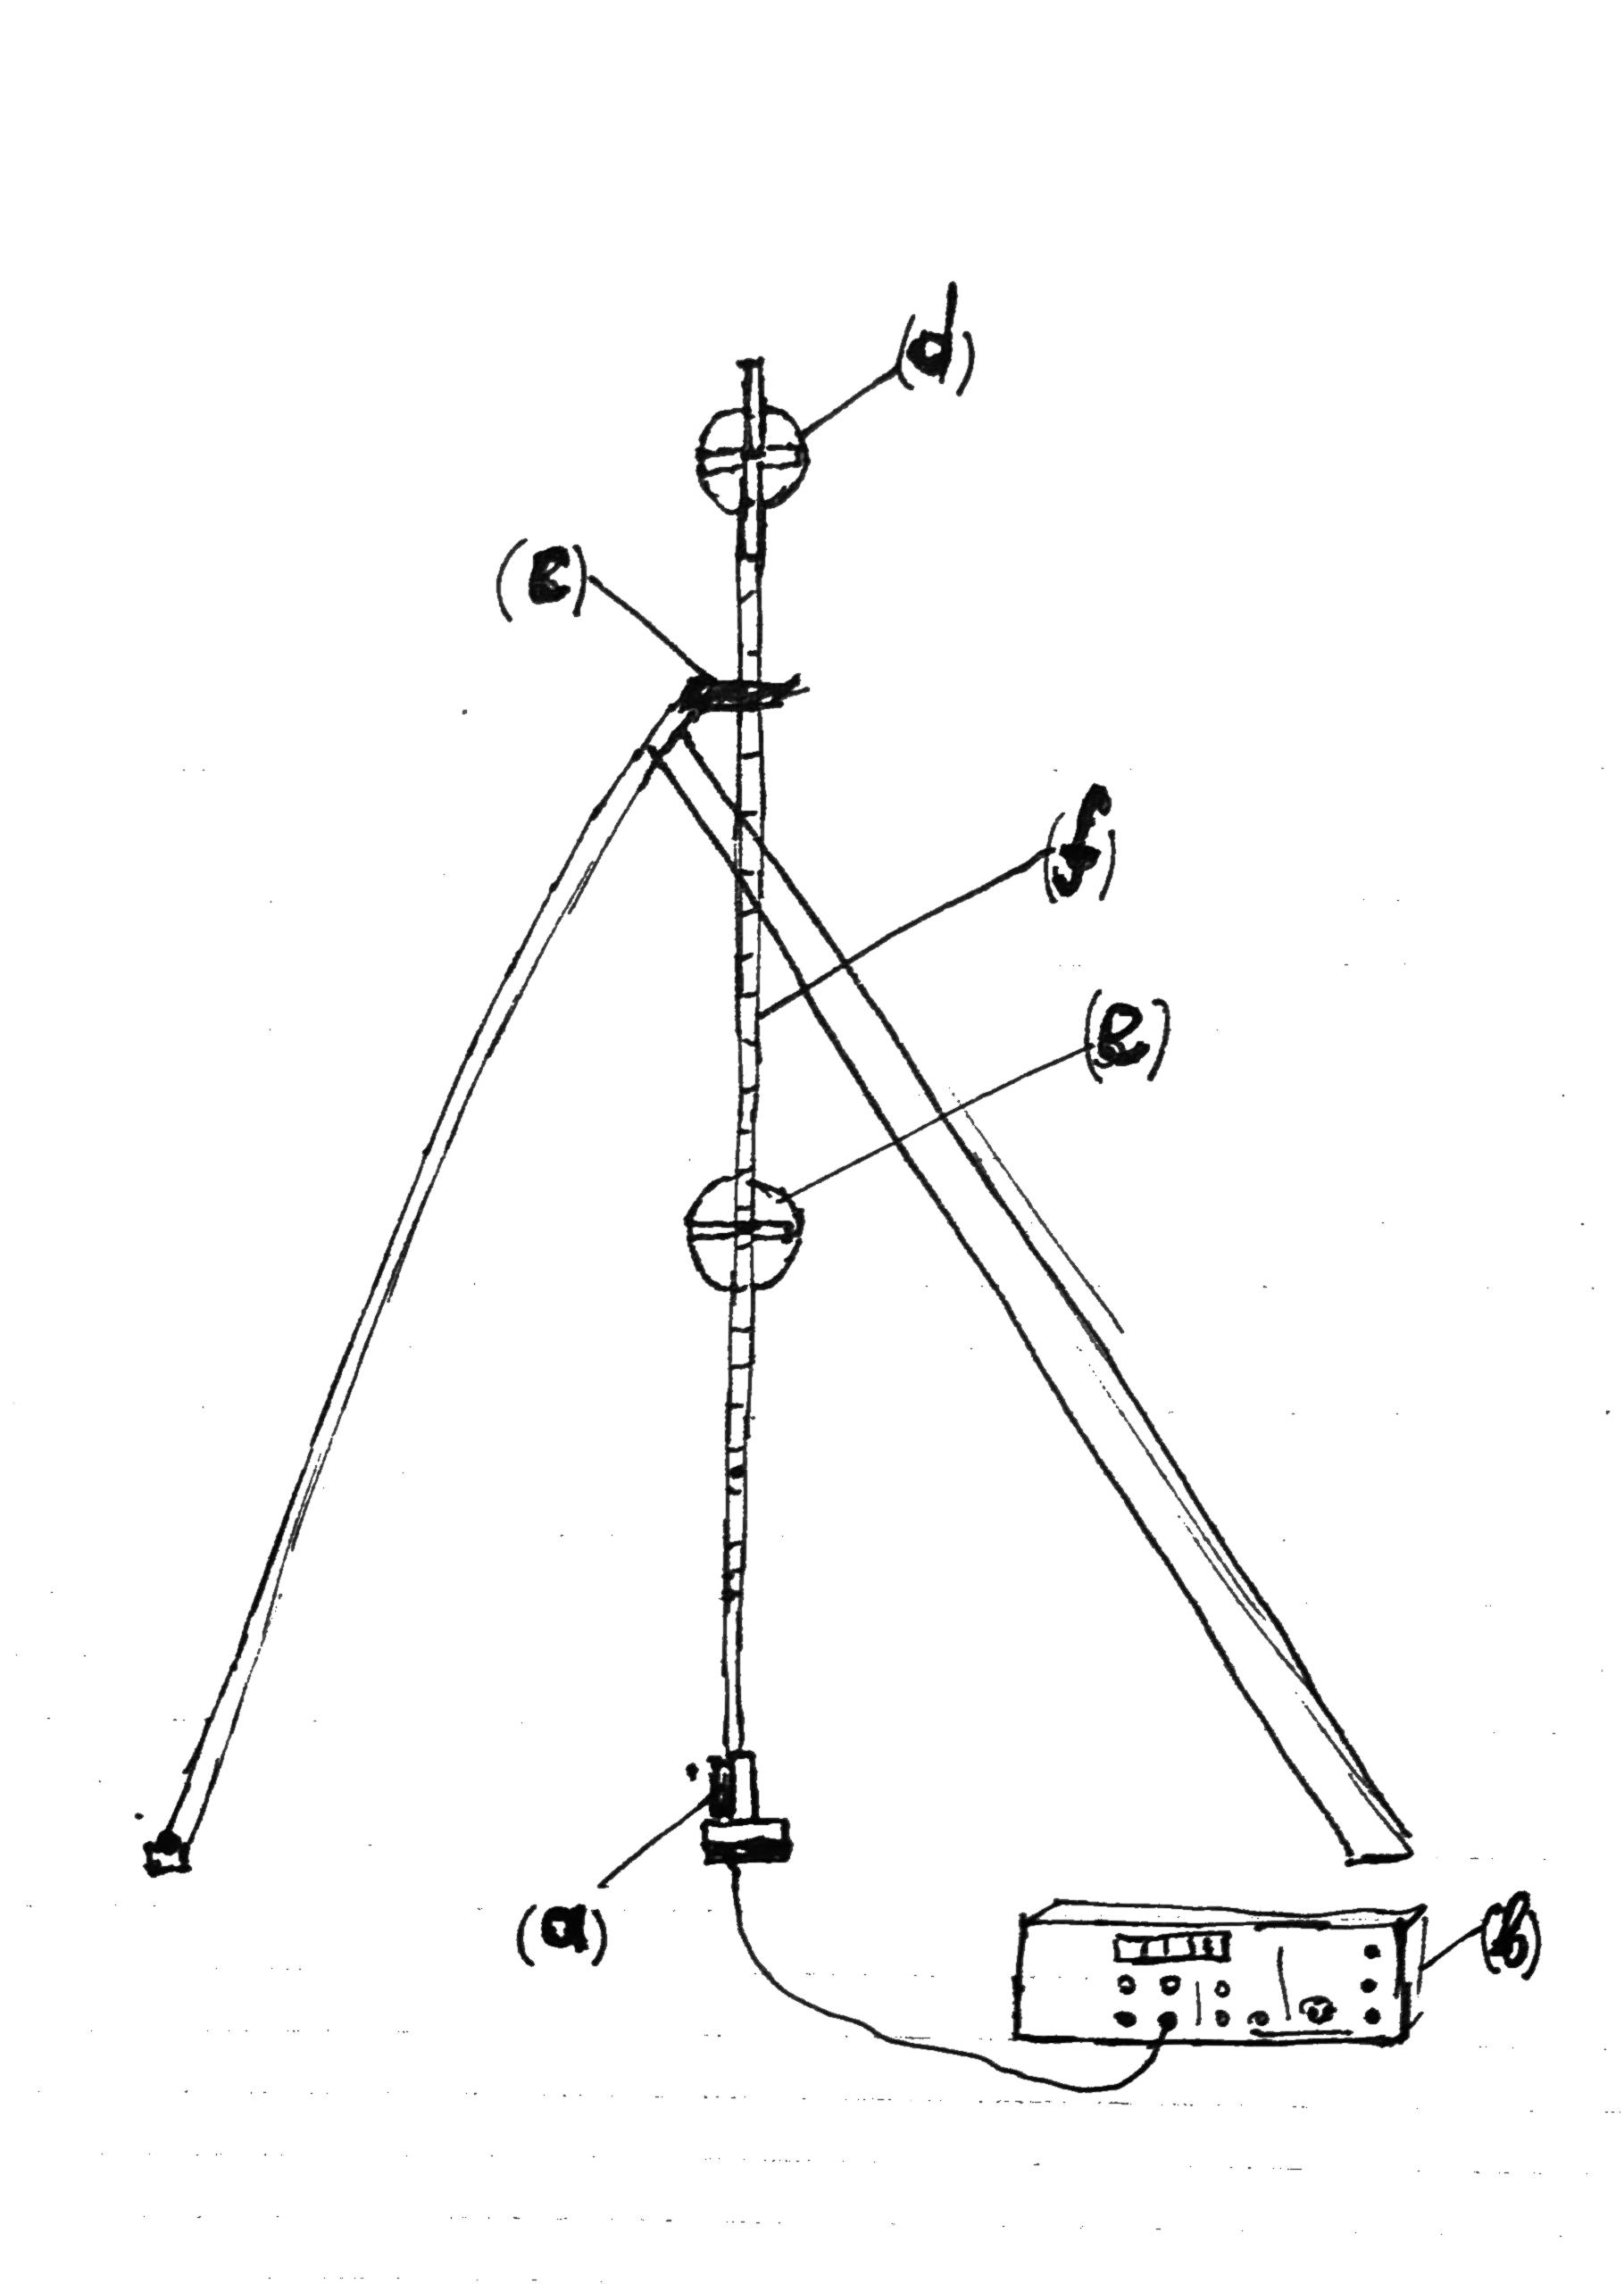
\includegraphics[scale=0.15]{scheme_1_24V.png}
	\begin{enumerate}
		\item Фотодатчик;
		\item Электронный секундомер;
		\item Точка подвеса;
		\item Тяжелый груз M1;
		\item Тяжелый груз M2;
		\item Стальной стержень.
	\end{enumerate}
	\item Результаты прямых измерений и их обработки (таблицы, примеры расчетов).
	\begin{center}
		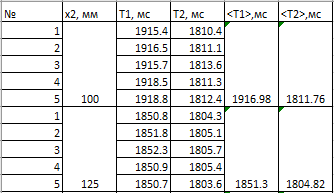
\includegraphics[scale=1.25]{table1_1_24V.png}\\
		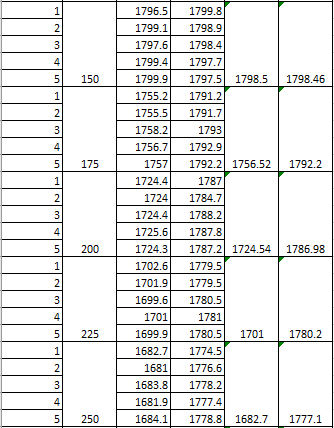
\includegraphics[scale=1.25]{table2_1_24V.png}\\
		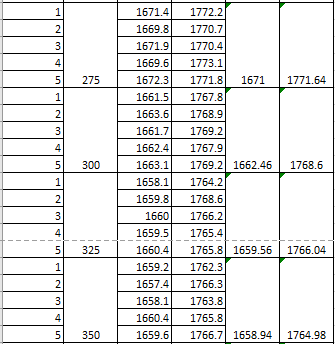
\includegraphics[scale=1.25]{table3_1_24V.png}\\
		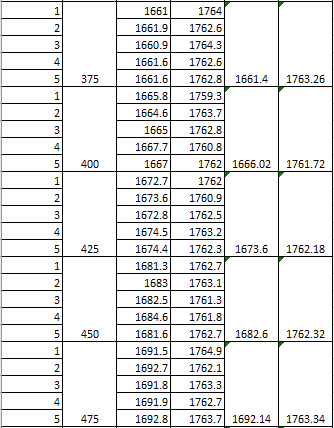
\includegraphics[scale=1.25]{table4_1_24V.png}\\
		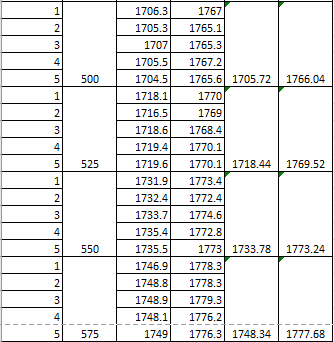
\includegraphics[scale=1.25]{table5_1_24V.png}\\
		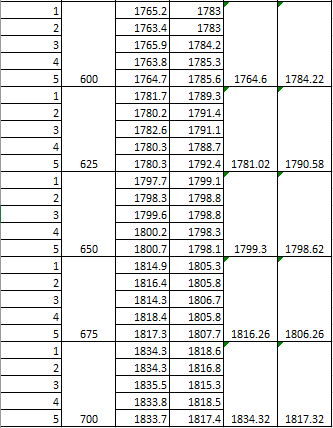
\includegraphics[scale=1.25]{table6_1_24V.png}\\
	\end{center}
	$$\left\langle T\right\rangle=\frac1N\sum_{i=1}^{N},$$
	\item Расчет результатов косвенных измерений (таблицы, примеры расчетов).
	$$l_{\mbox{пр}}=x_2+x'_2=800 \mbox{мм};$$
	$$g=\frac{4\pi^2l_{\mbox{пр}}}{T^2}=9,762 \frac{\mbox{м}}{c^2}$$
	\item Расчет погрешностей измерений (для прямых и косвенных измерений).
	$$\epsilon_g=\sqrt{{\left(\frac{2\Delta T}T\right)}^2+{\left(\frac{\Delta l_{\mbox{пр}}}{l_{\mbox{пр}}}\right)}^2}=0,00125$$
	$$\Delta_g=\epsilon_g\cdot g=0,012 \frac{\mbox{м}}{c^2}$$
	\newpage
	\item Графики.
	
	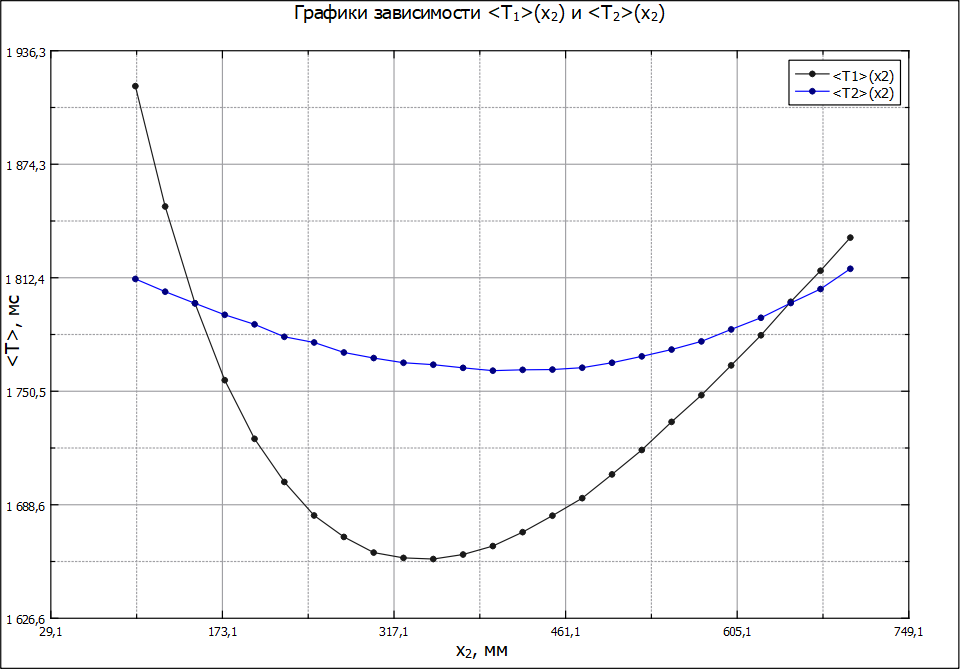
\includegraphics[scale=0.6]{graphic1_24V.png}
	\item Окончательные результаты.
	\begin{itemize}
		\item Графики зависимостей $<T_1(x_2)>$ и $<T_1(x_2)>$
		\item $g=9,762\pm0,012 \frac{\mbox{м}}{c^2},\ \delta_g=0,125\%$
	\end{itemize}
	\item Выводы и анализ результатов работы.
	\begin{itemize}
		\item Найденное ускорение свободного падения, даже с учетом погрешности, не соответствует значению ускорения свободного падения Земли ни на одной из широт. Это объясняется тем, что измерения проводились не на реальной физической модели, а на виртуальной.
		\item Больший вклад в погрешность ускорения свободного падения вносит погрешность приведенной длины, т.к, хоть период и входит в формулу ускорения свободного падения во 2-ой степени, а приведенная длина - в 1-ой, но относительная погрешность приведенной длины больше относительной погрешности периода в 25 раз.
	\end{itemize}
\end{enumerate}
\end{document}
